%% TODO (possibly): Use different formatting for code examples
%% \usepackage{listings}
%% \usepackage[scaled=0.81]{inconsolata}
%% \lstset{language=Python}
%% \lstset{showstringspaces=false}
%% [...]
%% \fontfamily{fi4}\selectfont
%% \begin{lstlisting}
%% [code goes here]
%% \end{lstlisting}
%% \fontfamily{cmr}\selectfont
%% [...]
%% This allows underscore, backslashes, and the like to be typed without needing to escape them.

% Releases:
% Version 0.0 for Hobbes 0.1.1.1-r21
% Version 0.1 for Hobbes 0.1.2.0-r22
% Version 0.2 for Hobbes 0.1.2.1-r23
% Version 0.3 for Hobbes 0.4-b31
% Version 0.4 for Hobbes 0.4-rc1
% Version 0.4.1 for Hobbes 0.4-rc9
% Version 0.4.2 for Hobbes 0.4.0.0-r38

\documentclass[12pt,letterpaper]{article}
\usepackage[utf8x]{inputenc}
\usepackage{ucs}
\usepackage{amsmath}
\usepackage{amsfonts}
\usepackage{amssymb}
\usepackage[pdftex]{graphicx}
\usepackage[margin=1in]{geometry}
\usepackage{hyperref}
\setcounter{secnumdepth}{5}
\author{Angus Lim}
\begin{document}

\begin{center}
\huge The Hobbes User Guide \\ \large Version 0.4.2
\end{center}

\tableofcontents
\pagebreak

\setcounter{section}{-1}



%
% Section 0
%
\section{Important Stuff}
\label{0}

This is the important stuff (as the section header implies), so here goes:

\setcounter{subsection}{-1}



%
% Section 0.0
%
\subsection{Software}
\label{0.0}

Hobbes runs on IronPython. IronPython runs on .NET. The Hobbes git repository, shamrock:s\_hobbes, includes IronPython 2.7.0.40 libraries and DLLs, so even if you don't have IronPython installed, you'll be fine.

If you don't have .NET installed though, that's a bit more serious. The .NET Framework is most definitely mandatory. The most recent version (.NET Framework 4) is strongly recommended; it \emph{might} work on older versions, but I've developed solely on .NET Framework 4 and you know how Microsoft is with backwards-(in)compatibility.

Lastly, you need a virtual COM port driver. But if you were using Tigger before, you should have had one beforehand.



%
% Section 0.1
%
\subsection{Running Hobbes}
\label{0.1}

I will attempt to make this as simple as possible.

\begin{itemize}
\item Clone the git repository from shamrock:s\_hobbes
\item Run Hobbes.bat in the cloned folder (preferably from a console)
\item ???
\item Profit!
\end{itemize}



%
% Section 0.2
%
\subsection{Why is he counting from 0 anyway?}
\label{0.2}

I'm a computer scientist.



%
% Section 1
%
\section{The Actual Introduction Now}
\label{1}

\textbf{Hobbes} (I haven't thought of anything it could stand for) is a program that communicates with a device through a serial port; more specifically, with Icron boards. It is written in IronPython, and runs on top of an IronPython environment. As a result, it is rather good at Python scripting. (This short introduction will do for now.)



%
% Section 2
%
\section{Supported boards}
\label{2}
Hobbes is designed solely for Goldenears (GE) support. Lionsgate (LG1) is also fully supported, as Hobbes contains Stewie file support as of version 0.4-rc1. If you have an older version of Hobbes, Hobbes will still be able to send iCommands to, receive iLogs from, and flash (using XMODEM) an LG1 board; it just won't be able to bootload them. Any other board hasn't been tested on Hobbes, and support would probably be somewhat icky for them.



%
% Section 3
%
\section{Using Hobbes}
\label{3}

This is probably the part of the guide you're looking for.

\setcounter{subsection}{-1}



%
% Section 3.0
%
\subsection{Starting Hobbes}
\label{3.0}

See \hyperref[0.1]{$\S0.1$}. Run Hobbes.bat. You should see a console start, and a startup window pop up.

If you have Hobbes 0.4-b30 or later, you may be prompted to load the previous session. This ``session'' is a JSON object of serial ports and .icron files. Upon (regular) exit, the values are taken from the Devices that were open and saved to Settings\textbackslash PreviousSession.hbs. If this file exists at startup time, and it's not an empty dictionary (meaning there were no Devices open from the previous session), you'll be prompted to load the previous session. If you select ``Yes'', Hobbes will create the necessary Device(s), connect to the serial port(s), and load the .icron file(s).



%
% Section 3.1
%
\subsection{Hobbes uses a Python interpreter}
\label{3.1}

\emph{Starting from Hobbes 0.4-b1, there has been a progression of GUI additions that mostly makes the following section obsolete. But this should still be of interest to you if you want to write Hobbes scripts, so I'll keep this here.}

If you have no Python experience, you might be a bit lost. This is a user's guide for Hobbes, not Python--but I'll include all the useful Python interpreter stuff you can do here:

\setcounter{subsubsection}{-1}



%
% Section 3.1.0
%
\subsubsection{Create and execute Python code}
\label{3.1.0}

Hobbes's interpreter is dynamic, so it runs Python code and such. It is, however, slightly different than a Python executable. The most important difference is that you'll probably have to prefix a command with ``print'' if you want to see its output, as shown below:

\begin{center}
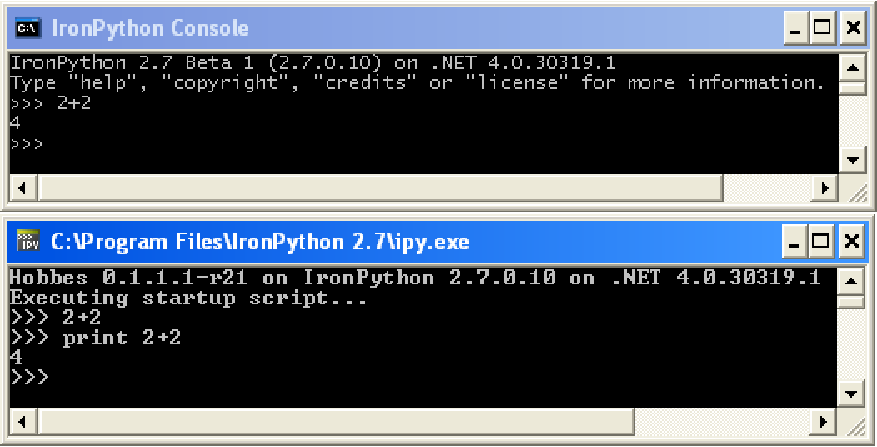
\includegraphics[scale=1]{interpreterdiff.pdf}
\end{center}

Disregarding that 2 + 2 = 5, of course (since Big Brother says so), note that the IronPython console did not require ``print'' to display 4 while Hobbes did. This apparently is a side effect of taking user input and executing it through an IronPython engine. But a) I don't want to spend the time figuring out when and when not to print and b) you might actually want suppressed output once in a while. In any case, if you want output and you don't see it, prefix your command with ``print'' and you should be fine.

(Python's code module would be very helpful here. Hobbes may use it in the future.)



%
% Section 3.1.1
%
\subsubsection{Use the horrific Windows console ``features''}
\label{3.1.1}

They're pretty bad. You can't select anything simply by holding a button and dragging. Or get any context menu when you right-click. There \emph{is} a bit of functionality, though; by clicking on the command prompt icon or right-clicking on the title bar, you get a little menu. And under ``Edit'', you'll see options for copying, marking (which you have to do before copying), and pasting.



%
% Section 3.1.2
%
\subsubsection{The dir() function}
\label{3.1.2}

\emph{This is a Python built-in function. If you know about this already, you can probably skip this.}
This function lists all the available functions and variables that can be called from a class, or an instance of a class. If you have, say, an iCommand class COM42\_ICMD, and you don't remember the available functions under that class, you can use dir():

\vspace{12pt}
\noindent $>>>$ print dir(COM42\_ICMD) \\ $[$'\_\_doc\_\_', '\_\_module\_\_', 'readMemory', 'readModifyWriteMemory', 'writeMemory']
\vspace{12pt}

(Note the usage of print.) The available functions are then readMemory, readModifyWriteMemory, and writeMemory. More on using these functions later.



%
% Section 3.1.3
%
\subsubsection{The \_\_doc\_\_ string}
\label{3.1.3}

(Again, users of Python will be familiar with this.)
This string simply gives information about the class or function it is declared in. Hobbes uses this most commonly in its auto-generated Python code (more on that later), where the help strings of iCommands are the \_\_doc\_\_ strings. These are the same strings that were in the iCommand selector form in Tigger. For example, continuing on the example in the previous section:

\vspace{12pt}
\noindent $>>>$ print COM42\_ICMD.readMemory.\_\_doc\_\_ \\ Read any memory address. Argument: full 32 bit address
\vspace{12pt}

(Again, print is required.) If you were to use Tigger's iCommand aliases and select component ICMD\_COMPONENT and command readMemory H, you would see this.



%
% Section 3.1.4
%
\subsubsection{Other stuff}
\label{3.1.4}

There's other cool Python stuff (getattr(), unordered arguments, et al.), but I've found the ones above most useful for Hobbes. Go through a Python tutorial if you want to learn more.

(By popular demand, a link! Chapters 2 to 4 in \url{http://diveintopython.org/toc/index.html} should help. That's what I used.)

\setcounter{paragraph}{1}
\setcounter{subparagraph}{4}
\subparagraph{This is just a pi reference, you can ignore this}
\label{3.1.4.1.5}



%
% Section 3.2
%
\subsection{Using a Device, the (sort of) deprecated way}
\label{3.2}

\emph{As the title of this section suggests, everything in this section has been mostly superseded by GUI windows as of the Hobbes 0.4 beta stream. However, you should still read through this section if you're interested in writing scripts for Hobbes, since you'll have to do a bunch of low-level stuff in said scripts.}

Hobbes has a Device class that includes everything you need to communicate with an Icron board. Most importantly, it includes a .NET SerialPort class instance which connects to the external board.

\setcounter{subsubsection}{-1}



%
% Section 3.2.0
%
\subsubsection{Finding serial port names}
\label{3.2.0}

To create a Device that's actually useful, you'll need to find your serial port names. You could do this in Hobbes, where there are (at least) three methods:

\begin{itemize}
\item Using the .NET SerialPort class

The class has a nice static method that returns an array of all the available serial ports. I'll just use an example:

\vspace{6pt}
\noindent $>>>$ print SerialPort.GetPortNames() \\ Array[str](('COM13', 'COM37', 'COM42'))
\vspace{6pt}

Your serial ports are probably going to be different (mine definitely are), but you'll see the serial ports there.


\item Using the builtin function in Hobbes

Quite similar to the above method. The main difference is that a Python module (\_winreg in Python 2, winreg in Python 3) is used to find the serial ports. It's a bit slower than SerialPort.GetPortNames(), but it'd be helpful if you want to port Hobbes to something that doesn't use .NET.

\vspace{6pt}
\noindent $>>>$ print availablePorts() \\ $[$'COM13', 'COM37', 'COM42']
\vspace{6pt}

Note that a list is returned, instead of a .NET array of strings. By the way, don't do this on a Mac. Or enter ``sys.platform = `darwin'; availablePorts()''. You may be surprised at the output.


\item Being lazy and letting Hobbes do the work for you

Alternatively, you could create a Device with an errant port name:

\vspace{6pt}
\noindent $>>>$ dev = Device(``This is definitely not a valid port name'') \\ Invalid serial port. \\ Available serial ports: \\ COM13 \\ COM37 \\ COM42

\end{itemize}

In any case, you should have a list of serial port names now.



%
% Section 3.2.1
%
\subsubsection{Creating the Device, and doing useful things with it}
\label{3.2.1}

There are two ways of going about this: the hard way, and the easy way.

\setcounter{paragraph}{-1}



%
% Section 3.2.1.0
%
\paragraph{The hard way}
\label{3.2.1.0}

Obviously, not the recommended way. You should skip this section and go on to reading about the easy way. But here it is.

\begin{enumerate}
\item Create a Device instance:\\
$>>>$ dev = Device(``COM42'')\\
Port set to COM42\\
Loading default settings

\item Set the Device's interpreter and interpreter scope:\\
$>>>$ dev.interpreter = hobbes.Calvin\\
$>>>$ dev.interpreterScope = hobbes.CalvinScope

\item Connect to the serial port:\\
$>>>$ dev.connect()\\
02/16/11 12:50:57 Connected to port COM42: 115200 Bd, 8-N-1; handshake: None\\
(Of course, you're going to see a different timestamp.)

\item Add the Device to deviceList:\\
$>>>$ hobbes.devices[``COM42''] = dev

\item Load a .icron file for the Device:\\
$>>>$ hobbes.load(``COM42'', ``Z:\textbackslash \textbackslash designs\textbackslash \textbackslash goldenears\textbackslash \textbackslash working\textbackslash \textbackslash angusl\textbackslash \textbackslash \\
p\_goldenears\_sw\textbackslash \textbackslash goldenears\_fpga\_bin\textbackslash \textbackslash goldenears\_fpga.icron'')\\
Loaded .icron file successfully\\
Python code for serial port COM42 created
\end{enumerate}



%
% Section 3.2.1.1
%
\paragraph{The easy way}
\label{3.2.1.1}

\begin{enumerate}
\item Do everything that was done in the previous section in \emph{one step}:\\
$>>>$ hobbes.load(hobbes.addDevice(``COM42''), ``Z:\textbackslash \textbackslash designs\textbackslash \textbackslash goldenears\textbackslash \textbackslash \\
working\textbackslash \textbackslash angusl\textbackslash \textbackslash p\_goldenears\_sw\textbackslash \textbackslash goldenears\_fpga\_bin\textbackslash \textbackslash goldenears\_fpga.icron'')\\
Port set to COM42\\
02/16/11 12:50:57 Connected to port COM42: 115200 Bd, 8-N-1; handshake: None\\
Loaded .icron file successfully\\
Python code for serial port COM42 created
\end{enumerate}

As you may have figured out, hobbes.addDevice() is \emph{really} useful. It does a lot of the steps you would be doing manually in the previous section. In addition, it returns the argument you just passed in, so you can use it in hobbes.load(). Speaking of hobbes...



%
% Section 3.2.2
%
\subsubsection{What's ``hobbes'', anyway?}
\label{3.2.2}

Note this is ``hobbes'', not ``Hobbes'', the actual program. It's the instance of the HobbesInterpreter class that you work with in the console. If you're interested, in HobbesInterpreter.py there's the following code:

\vspace{12pt}
\noindent self.CalvinScope.SetVariable(``hobbes'', self)
\vspace{12pt}

This allows the interpreter to call its own functions. These are addDevice(), load(), removeDevice(), and the constructor. They all have doc strings, so figuring out what happens in each of the functions is left as an exercise. (Side note: yes, you could call the constructor! But do you really want to? The only thing you'd get out of it is a good ``yo dawg'' joke and nothing more.)

Anyway, I'll get back to stuff you can do with your shiny new Device.



%
% Section 3.2.3
%
\subsubsection{Auto-generated Python code}
\label{3.2.3}

You might have noticed this whenever you load a .icron file to the Device:

\vspace{12pt}
``Python code for serial port COM42 created''
\vspace{12pt}

What happened there? Well, before this, the load() function of the Device was called. This called bsdtar.exe a bunch of times to extract icron\_header, icomponent, icmd, etc. After this, Python code is created, compiled, and executed, assuming the .icron file loaded.

I will spare you the gory details of what happens, and instead go on to what you could use the auto-generated Python code for:



%
% Section 3.2.4
%
\subsubsection{Sending iCommands}
\label{3.2.4}

As with creating a Device, there are some different ways of doing this. In all examples, I will use the iCommand of the Icron board connected to port COM42 to read the memory address at 0x00000000.

\setcounter{paragraph}{-1}



%
% Section 3.2.4.0
%
\paragraph{Self-torture}
\label{3.2.4.0}

Don't do it this way. Just don't.

\noindent $>>>$ print dir(COM42\_ICMD) \\ $[$'\_\_doc\_\_', '\_\_module\_\_', 'readMemory', 'readModifyWriteMemory', 'writeMemory'] \\ $>>>$ print hobbes.devices[``COM42''].iComponents \\ $[$\emph{All} of the iComponents are printed here] \\ $>>>$ for cmd in hobbes.devices[``COM42''].iCommands[``ICMD\_COMPONENT'']: \\ ... \indent print cmd \\ \# This is done to find the index of the readMemory iCommand within the list of iCommands \\ \# for ICMD\_COMPONENT. \\ readMemory \\ writeMemory \\ readModifyWriteMemory \\ $>>>$ hobbes.devices[``COM42''].iCommands[``ICMD\_COMPONENT''][0].send(0) \\ \# In DeviceWindow: \\ \# ``02/16/11 14:42:49 ICMD: UsrLog: Read address 0x00000000: value 0x033fffc0''
\vspace{12pt}

This is why I made Python code. I'm not going to bother explaining what's done here (except for the fact I made some comments). Still, the iComponents list may be useful if you need to see all of them at the same time.



%
% Section 3.2.4.1
%
\paragraph{Utilizing the Python code, Method I}
\label{3.2.4.1}

This involves creating an instance of one of the classes in the auto-generated Python code.

\noindent $>>>$ icmd = COM42\_ICMD() \\ $>>>$ icmd.readMemory(0) \\ \# In DeviceWindow: \\ \# ``02/16/11 14:42:49 ICMD: UsrLog: Read address 0x00000000: value 0x033fffc0''



%
% Section 3.2.4.2
%
\paragraph{Utilizing the Python code, Method II}
\label{3.2.4.2}

This is similar to Method I in the immediately preceding section, but no class instance is required this time:

\noindent $>>>$ COM42\_ICMD.readMemory(0) \\ \# In DeviceWindow: \\ \# ``02/16/11 14:42:49 ICMD: UsrLog: Read address 0x00000000: value 0x033fffc0''
\vspace{12pt}

As you can tell, either method using Python code is much easier to remember and enter than the first one by far.

I should probably say \emph{where} to enter these commands. Either the main Hobbes console or the input textbox of the DeviceWindow that pops up after a Device connects is acceptable--they both send Python code to the same interpreter (which, of course, I had to name Calvin). Currently, the only real good reasons that you should use the DeviceWindow instead of the console is that you can load Python scripts into the textbox with the ``Load...'' button, and copy/paste/cut is supported. With the main console, you have some functional history available, i.e. you can access previously-entered commands with the arrow keys. But of course, in either case, it's much easier to execute scripts than Tigger.

And I should say how to enter these commands, too. The class name (COM42\_ICMD in the previous examples) is derived from a) the serial port name the Device is connected to and b) the iComponent name. So you have, in order:

\begin{enumerate}
\item the serial port name (``COM42'' in the previous example);
\item an underscore; and
\item the iComponent name, without ``\_COMPONENT'' (``ICMD'' in the previous example).
\end{enumerate}

In each of these classes, there are functions corresponding to each iCommand. Continuing with COM42\_ICMD, one of the available iCommands is readMemory, and so you would call it like a Python function of a class (which it is!): COM42\_ICMD.readMemory().

(Caveat: iComponents without any iCommands don't have auto-generated Python code for them. Frankly, there's no use for them.)

With COM42\_ICMD.readMemory(), you can read the \_\_doc\_\_ string (see \hyperref[3.1.3]{$\S3.1.3$}). And you could do Python stuff with it, as it is a Python function. You could even use \_\_call\_\_, although it'd be completely inane as you can just call readMemory() with its argument! But anyway, you probably don't want to bother with all that (I didn't either). The \_\_doc\_\_ string should help you figure out how to send the iCommand: just enter COM42\_ICMD.readMemory(0) to read 0x00000000. And COM42\_ICMD.readMemory(0x30000000) to read 0x30000000. And so on. Hexadecimal numbers are supported as well as decimal numbers; don't use strings though, unless there's a boolT argument that only accepts ``TRUE'' or ``FALSE'' (actually, the quotation marks are optional for boolT arguments). If you avoid strings, you should be able to avoid raising any exceptions. Of course, mind the argument type; you won't get away with entering -42 for a uint32 argument type, and you'll definitely raise an exception by doing that.

\emph{If you don't have Hobbes 0.4-b5 or later, the following won't apply to you.}
The variable ``currentDevice'' contains the name of the serial port that sends code to Calvin. So if you have two DeviceWindows, say one connected to COM13 and the other to COM37, entering ``print currentDevice'' from the latter will print ``COM13'' to the console, while ``COM37'' will be printed for the latter.

Also, there is a function get\_iCommand() (as of Hobbes 0.4-b6) that takes a serial port name, iComponent name, and function name as arguments, and returns the iCommand corresponding to the arguments. You can combine this with currentDevice to dynamically retrieve iCommands without dependency on port names:

\vspace{12pt}
\noindent $>>>$ get\_iCommand(currentDevice, ``ICMD'', ``readMemory'')(0) \\ \# In DeviceWindow: \\ \# ``02/16/11 14:42:49 ICMD: UsrLog: Read address 0x00000000: value 0x033fffc0''


%
% Section 3.2.5
%
\subsubsection{Receiving iLogs}
\label{3.2.5}

Bytes sent from the serial port are received. Assuming you aren't bootloading/flashing the board, the bytes are sent to a function that parses them into an iLog message. Once a message is complete, it is output to the DeviceWindow with a nice timestamp. For more information on modifying output and scrolling the output textbox, see \hyperref[3.3.2]{$\S3.3.2$}.

Note that if an unknown byte is received, the console will output a message saying an unknown byte was received, along with the actual byte. I've noticed this happening when I cut power to a board, and somehow 0's are received. Sometimes there are 1's and 2's as well. Sometimes an unknown iLog is received as well. This might happen during startup of a board, when two 252 bytes are sent for some reason. Hobbes will figure out that there sure aren't 253 iComponents, and output a message to the console saying that an unknown iLog was received, and the bytes comprising that iLog in order. Hobbes is also very helpful, labelling each of the bytes according to their meaning in the iLog, i.e. labels like ``Header byte'', ``Component index'', ``Message index'', and so on.



%
% Section 3.2.6
%
\subsubsection{Sending iCmdResps}
\label{3.2.6}

\emph{This is only supported with GE version 2 .icron files and up. If you're not using those, this section will be useless to you.}

iCmdResps are pretty neat structures that intertwine an iCommand and an iLog together. Its function is quite simple:

\begin{enumerate}
\item Send an iCommand.
\item Wait for a specific iLog; if it doesn't come in time, timeout.
\item Parse the iLog as usual.
\item Get a specific argument from the iLog.
\item Return the argument.
\end{enumerate}

Sending one is similar to an iCommand.

\noindent \emph{Don't do this:} \\ $>>>$ print hobbes.devices[``COM42''].iCmdResps[``ICMD\_COMPONENT''][0].respSend(0) \\ 5452888 \\ \# In DeviceWindow: \\ \# ``02/16/11 16:36:04 ICMD: UsrLog: Read address 0x00000000: value 0x033fffc0''
\vspace{12pt}

\noindent \emph{Do this:} \\ $>>>$ print COM42RESP\_ICMD.read32(0) \\ 5452888 \\ \# In DeviceWindow: \\ \# ``02/16/11 16:36:04 ICMD: UsrLog: Read address 0x00000000: value 0x033fffc0''
\vspace{12pt}

I won't bore you with everything I said before regarding sending iCommands, because sending an iCmdResp is basically the same thing. The only difference is that the port name is immediately followed with ``RESP'' before the underscore. And the iCmdResp is named read32, not readMemory (although the iCmdResp \emph{calls} the readMemory iCommand).

That ``5452888'' is the returned value of read32(). If you check, the hexadecimal value of that is 0x033fffc0, which happens to be the value we read! Currently, calculating checksums might not be too exciting (and probably won't work, if you manage to cause a fatal error while reading memory). But iCmdResps to come should be very exciting.



%
% Section 3.2.7
%
\subsubsection{Bootloading and flashing}
\label{3.2.7}

Click the ``Bootload'' button. Or the ``Flash'' button. That's all there is to it.

You might want to bootload/flash in a script, so I should mention that the function being called for XMODEM sending is sendFileByXMODEM() in the XMODEM module. The function takes two arguments: the first being the Device to flash to, and the second being the name of the file to send, as specified in the .icron file. (For example, to send flash\_writer.bin you would enter ``flash\_writer'' or ``flash\_writer2'' as the second argument, depending on whether the board is LG1 or GE.) If for any reason the flashing of the file fails, the function will return False; if the flashing succeeds, it will return True. Note that the difference between clicking ``Bootload'' and clicking ``Flash'' is that clicking the latter will first send the first iCommand listed under TOPLEVEL\_COMPONENT (assumed to be xmodem\_new\_image) before beginning flashing of the flash writer, then the firmware. So if you have a test harness loaded, and you want to get back to main firmware, you'll want to manually reset the board to bootload mode, as there probably wouldn't be an iCommand available to start sending NAKs.

As of Hobbes 0.4-rc1, Stewie files are now supported; ergo, LG1 bootloading is now possible. The function called to send a Stewie file is sendFileByStewie() in the Stewie module; just like its XMODEM counterpart, it takes a Device and file name as parameters. The file name should always be ``flash\_writer'', as this corresponds to flash\_writer.icr in all versions of LG1 .icron files.

There are a couple of interesting things that may happen when you're bootloading an LG1 board:

\begin{itemize}
\item When an LG1 board is powered on into bootload mode, it will send a bunch of bytes through the serial port signifying that the bootloader is running. Hobbes will print a message when these certain bytes are received; however, on occasion the board decides to throw in a high-value byte before the bootloader bytes. As a result, Hobbes may show messages saying an exception was raised, but in reality the board is in bootloading mode. You can either reset power until you see the nice message stating a Device is in bootloading mode, or just go ahead with clicking ``Bootload''. It doesn't really matter.

\item When the Stewie file is transferred successfully, the Device will spit out a bunch of bytes again, consisting of a CR LF, the letters ``OK'', and another CR LF. Hobbes will also print out a neater message here, saying that bootloading was OK, but if the weird-exception-raised-thingy described above had happened, you'll see two unknown byte received messages: one for 13 and one for 10. No big deal, I hope.
\end{itemize}



%
% Section 3.2.8
%
\subsubsection{Changing Device settings}
\label{3.2.8}

Currently, the only Device settings are serial port settings. I don't see any reason why you would need to change the default settings, so don't.



%
% Section 3.2.9
%
\subsubsection{Printing}
\label{3.2.9}

When you use the print statement, regardless of whether the command was entered in the console or a DeviceWindow, the output will always go to the console. This is by design. I'm too lazy to redirect sys.stdout based on where a command was entered, so there is one function to print to console, one function to print to an arbitrary DeviceWindow, a different function to print to a different DeviceWindow, and so on. The functions to print to DeviceWindows are named after the serial ports they are connected to. The function name is the serial port name followed by ``\_OUT''. So for a Device connected to COM42, the function to print ``hello world'' to its output textbox would be ``COM42\_OUT(`hello world')''.

\emph{Note: before Hobbes 0.4-rc9, the function would be ``COM42\_out()'', with lowercase ``out''.}



%
% Section 3.3
%
\subsection{Using a Device, the mouse-intensive way}
\label{3.3}

This section will pretty much describe the exact same things as \hyperref[3.2]{$\S3.2$} does, with the exception that all the GUI components are used instead. So if you don't want to write any scripts for Hobbes, then you'll just want to read this section.

\setcounter{subsubsection}{-1}



%
% Section 3.3.0
%

\subsubsection{Creating the Device, and loading a .icron file for it}
\label{3.3.0}

As of Hobbes 0.4-b1, there is no longer any need to find out which serial ports you have manually. Hobbes does it for you!

Currently, the startup window (the one with an actual picture of Hobbes) does nothing more than create a Device and load a .icron file for it. There are two parameters:
\begin{itemize}
\item The serial port to connect to. This is why you don't need to figure out which ports you have! Also, Hobbes 0.4-b7 and later have a refresh button, so if you add or remove a serial port, you only have to hit the button to see a repopulated list.
\item The .icron file to load. Clicking the open button will open a dialog where you can select your .icron file. (Note you can resize this dialog, so you can actually read all of those ridiculously long paths.) You could also edit the path in the textbox. In any case, whatever's in the textbox is the path used when loading the .icron file.
\end{itemize}

Upon clicking ``Add Device'', a DeviceWindow will pop up after a while, and its title will change to include the path of the .icron file that was loaded. This assumes that you entered a valid serial port and .icron file path, of course.

Hobbes 0.4-rc22 added a ``Load .icron file'' button. This allows the user to change .icron files of Devices that already exist, so there is no need to close and reopen the DeviceWindow. Just make sure the ``Device:'' entry is the serial port whose .icron file you want changed, select the new .icron file to load, and hit ``Load .icron file''.



%
% Section 3.3.1
%
\subsubsection{Sending iCommands}
\label{3.3.1}

If you have an open Device, and Hobbes 0.4-b11 or later, click ``iCommands'' on the bottom toolbar. A window will open.

This window, which I will henceforth refer to as the ``iCommandWindow'', has quite a few useful features. Of course, they all pertain to iCommands, hence the title of this section.

If you've used Tigger before, you should be somewhat familiar with this procedure. First select the iComponent on the far left (but note that unlike Tigger, you can see all the components at once, and you can sort them alphabetically!). If there are iCommands for the selected iComponent, they will be shown in the box labelled ``Functions:'' to the immediate right of the iComponent box. Once you select a function (no plan for alphabetical sorting here), a bunch of stuff on the right will be populated, or re-populated.
\begin{itemize}
\item If there are any arguments required by the iCommand, the argument boxes will be enabled. How many are enabled corresponds to the number of arguments required. Also, the type of each argument is displayed below each enabled box. Note that everything will be a number, except arguments of type boolT. They must be either ``TRUE'' or ``FALSE''.
\item The help box will contain the help string of the iCommand.
\item The code box will contain the Python code used to send the iCommand...but if you're not interested in scripting, you can ignore this.
\end{itemize}

Once you've entered all your arguments, you can do one of two things:
\begin{itemize}
\item Execute the code. This does some fancy stuff that ultimately results in bytes being sent to the Device's serial port. But you're just clicking one button, you lazy dog.
\item Save the code to one of the buttons below. This is similar to Tigger's alias buttons. You'll probably want to set the ``Save to button'' and ``Text'' fields--the former sets which button to save to, with a range from 1 to 9 (counting left to right, top to bottom), and the latter sets the text on the button that the code will be saved to.

A warning: if you save some things to all nine buttons, and then accidentally close the iCommandWindow, your aliases will be gone! Once you reopen the window, none of them will be there anymore. I may fix this eventually, but for now just make sure you don't accidentally close windows. And make sure you use the save/load aliases functions. Clicking ``Save aliases...'' will open a dialog where you can save your aliases (comprising of the text and code for each button) to a file. Clicking ``Load aliases...'' will open a dialog where you can load your aliases.
\end{itemize}




%
% Section 3.3.2
%
\subsubsection{Receiving iLogs}
\label{3.3.2}

Fully parsed iLogs are printed to the upper textbox (henceforth referred to as the output textbox). As of Hobbes 0.4-b13, there are two checkboxes on the toolbar immediately below the output textbox that control output:

\begin{itemize}
\item The ``Suspend iLogs'' checkbox. This prevents iLogs from being printed, and saves them to a cache (it's a bit more complicated than that, but you won't need to know here). As soon as you uncheck this, the suspended iLogs are all displayed at once, unless you've disabled some of them--more on that later.
\item The ``Auto Scroll'' checkbox. This scrolls the textbox to the bottom automatically, as you may expect. Note that .NET is quirky and if you have focus on the output textbox (i.e. you've clicked inside of it), it's going to scroll to the bottom automatically regardless of whether ``Auto Scroll'' is clicked or not.
\end{itemize}

Hobbes 0.2.0.0-r33 added the iLogWindow, a window that is opened from a DeviceWindow and allows manipulation of the display of iLogs. This is somewhat similar to the iCommandWindow: to access individual iLogs, select an iComponent from the leftmost list (which can be sorted alphabetically). Assuming there are iLogs for your chosen iComponent, they will show up in the rightmost list. You can select as many iLogs as you want in this list to modify them all at once. There are two settings for an iLog:

\begin{itemize}
\item The font used to display the iLog. By clicking ``Font...'', you can modify the font itself, and its style, size, and colour. There is a preview textbox on the bottom of the iLogWindow, where you can see what the iLog will look like.

Note: the default font used is Consolas. You may not have it. If you see a default font displayed that is definitely not monospaced, then you don't have it.
\item Whether the iLog is displayed at all. This is controlled by the ``Enable iLog'' checkbox. If unchecked, the iLog(s) selected will not be displayed at all in the output textbox.
\end{itemize}



%
% Section 3.3.3
%
\subsubsection{Sending iCmdResps}
\label{3.3.3}

See \hyperref[3.2.6]{$\S3.2.6$} for iCmdResps. Why aren't they here? If you're using Hobbes only for Tigger-like functionality, parsing an iLog to return a value to a function really isn't that useful. Creating a GUI for iCmdResps would be completely unnecessary. And you'll only be using iCmdResps if you're scripting, and this is the non-scripting section.



%
% Section 3.3.4
%
\subsubsection{Bootloading and flashing}
\label{3.3.4}

Click the ``Bootload'' button if you see the Device sending NAKs. Or the ``Flash'' button if you know for sure that the first iCommand under TOPLEVEL\_COMPONENT is named xmodem\_new\_image.

But if you're connected to an LG1 device, and you have Hobbes 0.4-rc1 or later, click ``Bootload'' if you know it's in bootloading mode and ``Flash'' if it's in regular operation. See \hyperref[3.2.7]{$\S3.2.7$} if you want to know more (but you probably don't).



%
% Section 3.4
%
\subsection{Exiting Hobbes}
\label{3.4}

You have a few options:
\begin{itemize}
\item Hitting the X button in the console
\item Entering ``exit'' in the console
\item Entering Ctrl-D in the console (the real EOF key combination, of course)
\end{itemize}



%
% Section 4
%
\section{A conclusion of sorts}
\label{4}

This is a temporary paragraph. Its only purpose is to serve as a reminder that this conclusion is far from complete, only the really important information needed to conclude the document is included, and ideally it will progressively become more and more complete.

And if you think that this sounds a tiny bit familiar, good for you.



\end{document}